\documentclass[12pt]{article}
\usepackage{amsmath,amsthm, amsfonts, amssymb, amsxtra, amsopn}
\usepackage{pgfplots}
\pgfplotsset{compat=1.13}
\usepackage{pgfplotstable}
\usepackage{colortbl}

\begin{document}

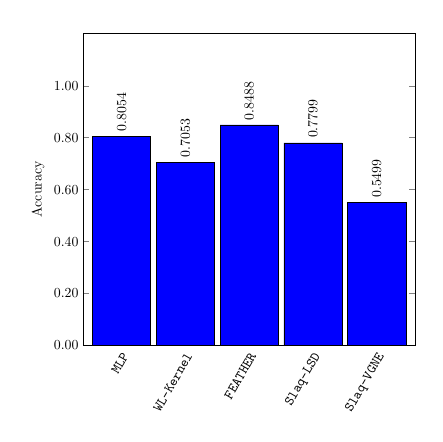
\begin{tikzpicture}[scale=0.5, every node/.style={scale=1.0}]
    \begin{axis}[
        width  = 0.825*\textwidth,
        height = 9.5cm,
        ymin=0.0,ymax=1.2,
        ytick={0,0.2,0.4,0.6,0.8,1.0},
        major x tick style = transparent,
        ybar=5*\pgflinewidth,
        bar width=42.0pt,
%        ymajorgrids = true,
        ylabel = {Accuracy},
        symbolic x coords={
MLP,
WL-Kernel,
FEATHER,
Slaq-LSD,
Slaq-VGNE
},
        xtick=data,
	y tick label style={
%		rotate=90,
    		/pgf/number format/.cd,
   		fixed,
   		fixed zerofill,
    		precision=2},
%	yticklabel pos=right,
%        xtick = data,
        x tick label style={
        		rotate=60,
		font=\tt,
		anchor=north east,
		inner sep=0mm
		},
%        scaled y ticks = false,
	%%%%% numbers on bars and rotated
        nodes near coords,
        every node near coord/.append style={rotate=90, 
        								   anchor=west,
								   /pgf/number format/.cd,
								   	fixed zerofill,
									precision=4
								   },
        %%%%%
%        enlarge x limits=0.03,
        enlarge x limits=0.15,
%        enlarge x limits=0.25,
        legend cell align=left,
        legend pos=south east,
%                anchor=south east,
%                anchor=south,
%                column sep=1ex
%        axis x line*=bottom
    ]
\addplot[fill=blue,opacity=1.00]
coordinates {
(MLP,0.8054)
(WL-Kernel,0.7053)
(FEATHER,0.8488)
(Slaq-LSD,0.7799)
(Slaq-VGNE,0.5499)
};
\end{axis}
\end{tikzpicture}

\end{document}